\documentclass[12,twoside]{TFG-GM}
%\usepackage[active]{srcltx}
\usepackage{amsthm,amsmath,amssymb,amsfonts,amscd}
\usepackage{graphicx}
\usepackage{enumerate}
\usepackage[all]{xy}
\usepackage{booktabs}
%\usepackage[usenames]{xcolor}
%\usepackage{fancyhdr}
\usepackage{minted}
%%%%%Author packages if necessary
\usepackage{hyperref}
\usepackage[spanish]{babel}

\usepackage[utf8]{inputenc}
\usepackage[T1]{fontenc}
\usepackage{environ}

\usepackage{tikz}
%\usetikzlibrary{arrows}
\usetikzlibrary{positioning}

\usepackage{pgfplots}
\pgfplotsset{compat=1.10}

\usepackage[nottoc]{tocbibind} %Adds "References" to the table of contents


% Theorem Environments: add extra ones at the end if you need it.

\newtheorem*{theoremA}{Theorem A}
\newtheorem{theorem}{Theorem}[section]

\newtheorem{proposition}[theorem]{Proposition}
\newtheorem{lemma}[theorem]{Lemma}
\newtheorem{corollary}[theorem]{Corollary}
\newtheorem{conjecture}[theorem]{Conjecture}

\theoremstyle{definition}
\newtheorem{definition}[theorem]{Definition}
\newtheorem{example}[theorem]{Example}

\theoremstyle{remark}
\newtheorem{remark}[theorem]{Remark}
\newtheorem*{remarknonumber}{Remark}
\newtheorem{observation}[theorem]{Observation}




%%%%%%%%%%%%%%%%%%
% macros/abbreviations: Include here your own.
%%%%%%%%%%%%%%%%%%

\newcommand{\N}{\ensuremath{\mathbb{N}}}

%%%%%%%%%%%%%%%%%%
% tikz config
%%%%%%%%%%%%%%%%%%


\tikzset{basic/.style={draw,fill=blue!20,text width=1em,text badly centered}}
\tikzset{input/.style={basic,circle}}
\tikzset{weights/.style={basic,rectangle}}
\tikzset{functions/.style={basic,circle,fill=blue!10}}
\tikzstyle{arrow}=[draw, -latex]

\makeatletter
\newsavebox{\measure@tikzpicture}
\NewEnviron{scaletikzpicturetowidth}[1]{%
  \def\tikz@width{#1}%
  \def\tikzscale{1}\begin{lrbox}{\measure@tikzpicture}%
  \BODY
  \end{lrbox}%
  \pgfmathparse{#1/\wd\measure@tikzpicture}%
  \edef\tikzscale{\pgfmathresult}%
  \BODY
}
\makeatother

% Body of document

\titol{ Wordnet y Deep Learning: Una posible unión}
\titolcurt{Short title}
\authorStudent{Raquel Leandra Pérez Arnal}
\supervisors{(name of the supervisor/s of the master's thesis)}
\monthYear{Month, year}

%\msc[2010]{Primary  	55M25, 57P10, Secondary 55P15, 57R19, 57N15.}

\paraulesclau{keyword1, keyword2, keyword3, ...}
\agraiments{
Thanks to...}


\abstracteng{This should be an abstract in english, up to 1000 characters.}

%%%%%%%%%
\begin{document}

\maketitle

\section{Estructura del TFG: }

\begin{itemize}
\item \textbf{Introducción (5 pags): }
\begin{itemize}
\item FNN (Explicar neural networks, me puedo inspirar en \url{https://upc-mai-dl.github.io/mlp-convnets-theory/})
\item CNN 
\item EMbeddings  (Transfer Learning)
\end{itemize}
\item \textbf{Related Work (10 pags):}
\begin{itemize}
\item FNE 
\item Wordnet 
\item imagenet 
\end{itemize}
\item \textbf{Approach }
\begin{itemize}
\item Hipotesis iniciales 
\item statistics 
\item insights 
\end{itemize}
\item \textbf{Analysis}
\begin{itemize}
\item De wordnet a imagenet: Dado el embedding hemos encontrado patrones con los distintos synsets que concuerdan con las hipótesis
\item De imagenet a wordnet: Dado el árbol sintáctico y los patrones anteriores podemos generar una distancia con la que representamos lo parecidos que son los siynsets para la imagen. 
\end{itemize}
\end{itemize}

%\section{Introducción}
\newpage
\section{Conocimientos previos}
%\subsection{Machine Learning}
%%- Que es ml y por que está de moda. 
%%- Un poco de historia
%En los últimos años(fecha) ha estado en alza todo lo relacionado con \textit{Machine Learning}, pero, que es realmente machine learning? 
%Machine Learning es una aplicación de la Inteligencia Artificial que provee sistemas de la habilidad de mejorar a partir de una experiencia sin ser explícitamente programados para ello. 
%
%Su crecimiento se debe a: 
%\begin{itemize}
%\item Aumento de la capacidad computacional de los ordenadores. 
%\item Aumento de la cantidad de datos disponibles, junto la necesidad de analizarlos. 
%\end{itemize}
%
%En nuestro caso concreto nos centraremos en la aplicación de diversos métodos de ML a el problema de clasificación de imágenes. 


\subsection{Redes Neuronales}
Una \textbf{red neuronal} es un modelo computacional inspirado en la forma de procesar información de las neuronas del cerebro. Las redes neuronales han generado una significativa cantidad de investigación e industria gracias a sus resultados en reconocimiento del habla, visión por computador y procesamiento de texto. Para dejar claro su funcionamiento explicaré primero el funcionamiento de una sola neurona, para después unirlo con las distintas arquitecturas posibles. 

\subsubsection{neurona}

La unidad de computación básica de una red neuronal es una \textbf{neurona}, también llamada nodo o unidad. Su función es recibir una entrada desde otros nodos y calcular una salida. 

Cada entrada (\textbf{x}) tiene asociado un peso, que es asignado en base a su importancia relativa a otras entradas. La neurona  aplica una función (\textbf{f}) a la suma ponderada de las entradas como muestra la figura: 
%\begin{center}
%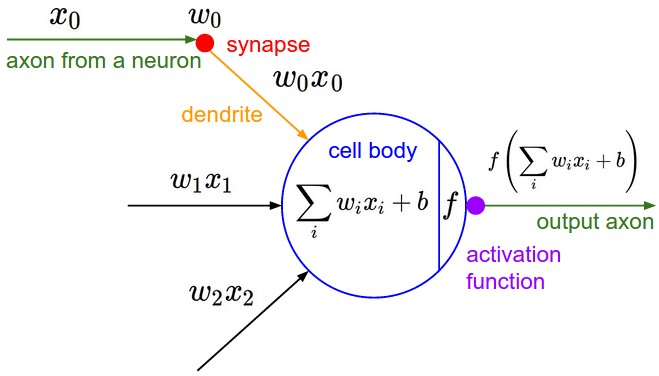
\includegraphics[width=0.5\textwidth]{Images/neuron_model.jpeg} 
%\end{center}
\begin{figure}[H]
\centering
 \begin{tikzpicture}
        \node[functions] (center) {$f$};
        \node[below of=center,font=\scriptsize,text width=4em] {Función de activación};

        \node[right of=center] (right) {};
            \path[draw,arrow] (center) -- (right);
        \node[functions,left=3em of center,text width=3em ] (left) {$\sum w_i x_i$};
            \path[draw,arrow] (left) -- (center);
        \node[weights,left=3em of left] (2) {$w_2$} -- (2) node[input,left of=2] (l2) {$x_2$};
            \path[draw,arrow] (l2) -- (2);
            \path[draw,arrow] (2) -- (left);
        \node[below of=2] (dots) {$\vdots$} -- (dots) node[left of=dots] (ldots) {$\vdots$};
        \node[weights,below of=dots] (n) {$w_n$} -- (n) node[input,left of=n] (ln) {$x_n$};
            \path[draw,arrow] (ln) -- (n);
            \path[draw,arrow] (n) -- (left);
        \node[weights,above of=2] (1) {$w_1$} -- (1) node[input,left of=1] (l1) {$x_1$};
            \path[draw,arrow] (l1) -- (1);
            \path[draw,arrow] (1) -- (left);
        \node[weights,above of=1] (0) {$w_0$} -- (0) node[input,left of=0] (l0) {$1$};
            \path[draw,arrow] (l0) -- (0);
            \path[draw,arrow] (0) -- (left);
        \node[below of=ln,font=\scriptsize] {Pesos};
        \node[below of=n,font=\scriptsize] { Entrada};
    \end{tikzpicture}
\end{figure}
Además de los elementos ya comentados tendremos un término de sesgo (\textbf{b}), cuya función consiste en proveer cada nodo con un valor entrenable que no dependa de la entrada. 

La salida de la neurona (\textbf{Y}) se calculara de la siguiente manera: 

$$
Y = f \left(\sum_i \omega_i x_i + b \right) 
$$

Llamaremos a \textbf{f} la \textbf{función de activación}, es una función no lineal cuyo propósito es introducir no linealidad a la salida de la neurona. Ésto ayuda a adaptar mejor el modelo a problemas reales, puesto a que estos raramente son lineales. 

Las funciones de activación más utilizadas son: 

\begin{itemize}
\item Sigmoide: $f(x)=\frac{1}{1+e^{-x}}$
\begin{figure}[H]
\centering
%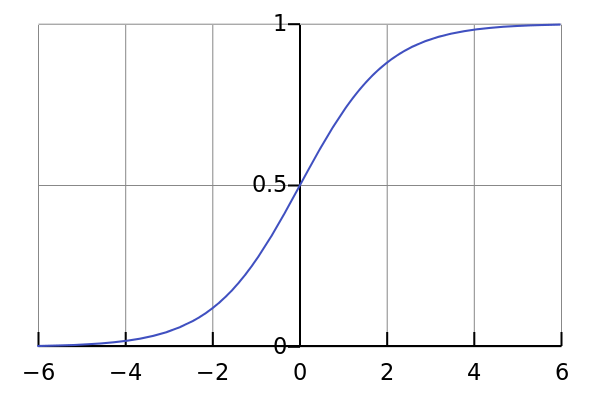
\includegraphics[width=0.5\textwidth]{Images/sigmoid.png} 
\begin{scaletikzpicturetowidth}{0.5\textwidth}
\begin{tikzpicture}[scale=\tikzscale]
    \begin{axis}[
        legend pos=north west,
        axis x line=middle,
        axis y line=middle,
        y tick label style={/pgf/number format/fixed,
                            /pgf/number format/fixed zerofill,
                            /pgf/number format/precision=1},
        grid = major,
        width=16cm,
        height=8cm,
        grid style={dashed, gray!30},
        xmin=-4,     % start the diagram at this x-coordinate
        xmax= 4,     % end   the diagram at this x-coordinate
        ymin= 0,     % start the diagram at this y-coordinate
        ymax= 1,     % end   the diagram at this y-coordinate
        %axis background/.style={fill=white},
        xlabel=$t$,
        ylabel=sig$(t)$,
        tick align=outside,
        enlargelimits=true]
      % plot the stirling-formulae
      \addplot[domain=-5:5, black, ultra thick,samples=500] {1/(1+exp(-1*x))};
      \addlegendentry{sig$(t)=\frac{1}{1+e^{-t}}$}
    \end{axis}
\end{tikzpicture}
\end{scaletikzpicturetowidth}
\end{figure}
\item Tanh: $f(x)=\frac{2}{1+e^{-2x}}-1$
\begin{figure}[H]
\centering
%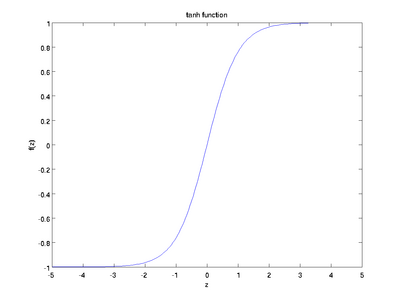
\includegraphics[width=0.5\textwidth]{Images/tanh.png} 
\begin{scaletikzpicturetowidth}{0.5\textwidth}
\begin{tikzpicture}[scale=\tikzscale]
    \begin{axis}[
        legend pos=north west,
        axis x line=middle,
        axis y line=middle,
        y tick label style={/pgf/number format/fixed,
                            /pgf/number format/fixed zerofill,
                            /pgf/number format/precision=1},
        grid = major,
        width=16cm,
        height=8cm,
        grid style={dashed, gray!30},
        xmin=-4,     % start the diagram at this x-coordinate
        xmax= 4,     % end   the diagram at this x-coordinate
        ymin= -1,     % start the diagram at this y-coordinate
        ymax= 1,     % end   the diagram at this y-coordinate
        %axis background/.style={fill=white},
        xlabel=$x$,
        ylabel=$tanh(x)$,
        tick align=outside,
        enlargelimits=true]
      % plot the stirling-formulae
      \addplot[domain=-5:5, black, ultra thick,samples=500] {2/(1+exp(-2*x)) - 1};
      \addlegendentry{$tanh(x)=\frac{2}{1+e^{-2x}}-1$}
    \end{axis}
\end{tikzpicture}
\end{scaletikzpicturetowidth}
\end{figure}

%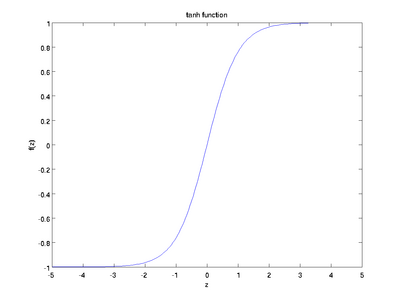
\includegraphics[scale=1]{Images/tanh.png} 
\item ReLU: $f(x)=max(0,x)$

\begin{figure}[H]
\centering
%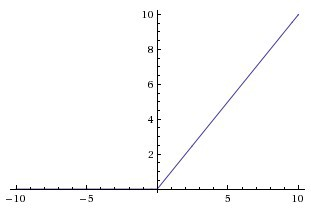
\includegraphics[width=0.5\textwidth]{Images/relu.jpeg} 
\begin{scaletikzpicturetowidth}{0.5\textwidth}
\begin{tikzpicture}[scale=\tikzscale]
    \begin{axis}[
        legend pos=north west,
        axis x line=middle,
        axis y line=middle,
        y tick label style={/pgf/number format/fixed,
                            /pgf/number format/fixed zerofill,
                            /pgf/number format/precision=1},
        grid = major,
        width=16cm,
        height=8cm,
        grid style={dashed, gray!30},
        xmin=-4,     % start the diagram at this x-coordinate
        xmax= 4,     % end   the diagram at this x-coordinate
        ymin= 0,     % start the diagram at this y-coordinate
        ymax= 4,     % end   the diagram at this y-coordinate
        %axis background/.style={fill=white},
        xlabel=$x$,
        ylabel=$relu(x)$,
        tick align=outside,
        enlargelimits=true]
      % plot the stirling-formulae
      \addplot[domain=-5:5, black, ultra thick,samples=500] {max(0,x)};
      \addlegendentry{$f(x)=max(0,x)$}
    \end{axis}
\end{tikzpicture}
\end{scaletikzpicturetowidth}
\end{figure}
%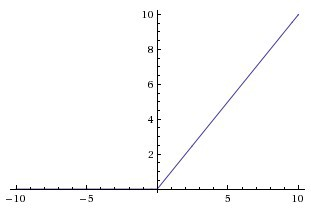
\includegraphics[scale=1]{Images/relu.png} 
\end{itemize}

%

Dotando una neurona de una función de pérdida en la salida podríamos convertirla en un clasificador lineal, pero la verdadera potencia del método viene dada al unir diversas neuronas en lo que llamaremos capas (layers).

\subsubsection{Organización por capas}
Las redes neuronales se modelizan como una colección de neuronas conectadas en un grafo acíclico, comúnmente organizado por capas. El tipo más común es el \textit{fully-connected layer}, en el que todas las neuronas de dos capas consecutivas están conectadas entre ellas, mientras que no comparten ninguna conexión con las de su propia capa, como muestra la figura. Si tenemos diversas capas ocultas diremos que se trata de una \textit{red profunda}.

\begin{center}
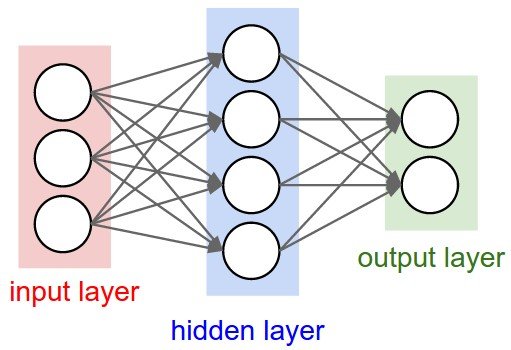
\includegraphics[width=0.5\textwidth]{Images/neural_net.jpeg} 
\end{center}
La red neuronal más básica la podemos dividir en: 
\begin{enumerate}
\item Nodos de entrada: Proveen la red de información del exterior, todo su conjunto se conoce como la capa de entrada. 
\item Nodos ocultos: Los nodos ocultos no tienen conexión directa con el exterior. Solo calculan y transfieren información de la entrada a la salida. La colección de los nodos ocultos se denomina las capas ocultas.
\item Nodos de salida: Colectivamente denominados nodos de salida y son responsables de la computación y transferencia de información al exterior. 
\end{enumerate}

Dos ejemplos de redes de este tipo serían el perceptron y el multilayer perceptron. 

Finalmente, queda explicar como entrenar los distintos parámetros para que se adapten a los datos. 

\subsubsection{Backpropagation}

El algoritmo de backpropagation empieza con un \textit{fordward pass} de los datos por toda la red, la predicción dada por la red se compara con la salida esperada 
y se calcula un error utilizando la función de pérdida. La pérdida calculada se utiliza para actualizar los pesos de la última capa, buscando los valores de éstos que la minimizan.

La complejidad reside en optimizar los pesos de las capas que no están conectadas directamente con la salida. Para resolver esto backpropagation utiliza la regla de la cadena, que permite calcular derivadas de capas previas, y de esta forma actualizar los pesos de las capas restantes. 

Tradicionalmente, el cambio e pesos se ha computado usando el algoritmo de optimización llamado Stochastig Gradient Descent, un método iterativo de minimización.

De esta forma, aplicando backpropagation iterativamente podemos estimar los pesos de todas las capas de una red neuronal para un problema dado.




\newpage

\subsection{Redes convolucionales}
%- Explicar el problema inicial (clasificación de imágenes) y por que es difícil.
%- Explicar que es una red convolucional 

Las redes convolucionales son muy similares a las redes neuronales explicadas, las mayores diferencias son que están basadas en un tipo especial de neuronas (las neuronas convolucionales) y que asume explícitamente que la entrada son imágenes, lo que permite añadir ciertas propiedades a la arquitectura. Esto permite hacer un \textit{fordward pass} más eficiente de implementar y reducir significativamente la cantidad de parámetros, nótese que cuantos más parámetros tenga una red, mayor subconjunto de datos de entrenamiento necesitamos para evitar tener sobreajuste.

Típicamente las neuronas convolucionales tienen una entrada limitada, es decir están conectadas solo a un subconjunto de las neuronas de la capa anterior. En contraste, las neuronas de una capa \textit{fully-connected} están conectadas a todas las neuronas de la capa anterior. La idea de convolución puede aplicarse a una entrada de cualquier dimensión. En este caso detallaremos el caso de datos en dos dimensiones, por ser el caso más común y por ser más fácil de entender. Una vez comprendida una convolución 2-dimensional, el lector puede extrapolar a tantas dimensiones como sea necesario.

%Para definir su conectividad de entrada, las neuronas convolucionales asumen la existencia de una cierta estructura en los datos. 
Para capturar patrones consistentes, espacialmente en un subconjunto de la entrada, las neuronas convolucionales están conectadas a un conjunto de neuronas de la capa anterior que definen parcelas cuadradas (en el caso de convoluciones de dos dimensiones).

\begin{center}
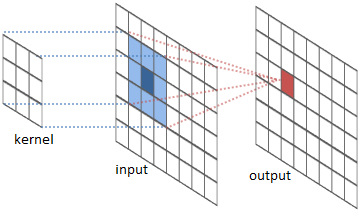
\includegraphics[width = 0.5\textwidth]{Images/convolution2.png} 
\end{center}


Por su conectividad limitada, las capas convolucionales pueden centrarse en una parcela particular de la entrada. El kernel(e.d, el conjunto de pesos) aprendido por esta parcela puede ser relevante para las otras parcela de la entrada, por tanto, podemos definir neuronas similares que utilicen el mismo kernel, pero que se enfoquen en otra parte de la entrada. Esta idea se conoce como "weight sharing",por que varias neuronas de la misma capa están definidas por un conjunto común de pesos, esto permite tener una considerable cantidad de neuronas utilizando los mismos parámetros. 

\begin{center}
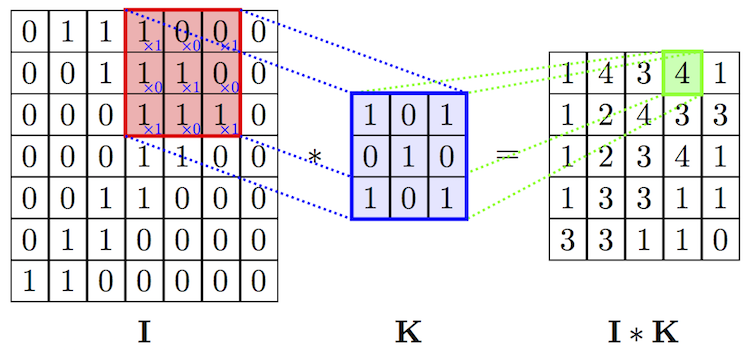
\includegraphics[width = 0.5\textwidth]{Images/convolve.png} 
\end{center}

Como ha sido descrito con anterioridad una red convolucional es una secuencia de capas, donde cada capa transforma un volumen de activaciones en otro a través de una función diferenciable los tipos de capa que se suelen utilizar en una red convolucional son: 
\begin{itemize}
\item Capa convolucional, capas adaptadas a imágenes en las que se comparten los pesos.
\item Capa completa, es el tipo de capa básico, explicado en el capítulo anterior. 
\item Pooling Layer, consiste en una capa que aplica una reducción matemática a su input(como una media o un max). El objetivo es facilitar a la red que reconozca datos que están relacionados en un sentido espacial (imágenes equivalentes en diferentes posiciones), además típicamente reducen el tamaño de la salida de la capa, lo que provoca una reducción de la complejidad de la red.
\end{itemize}

\begin{center}
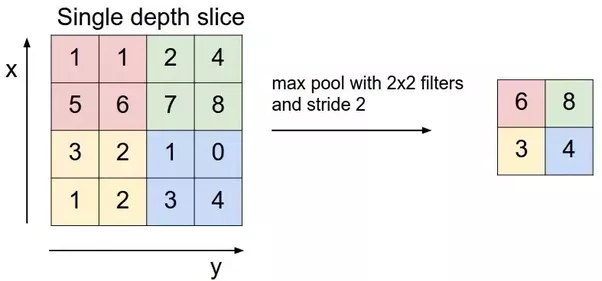
\includegraphics[width = 0.5\textwidth]{Images/pooling1.png} 
\end{center}

\newpage
\subsection{Transfer Learning}
%- Explicar que es transfer learning 

En la práctica pocas personas entrenan una red profunda desde cero(con inicialización aleatoria), puesto a que tienen unos requisitos bastante exigentes a la hora de entrenarla, los mayores problemas que puedes encontrar son: 
\begin{enumerate}
\item A causa de la gran cantidad de parámetros a entrenar que tiene una red profunda necesitas un \textbf{conjunto de datos de gran tamaño}.
\item El \textbf{coste computacional} de entrenar la red. 
\item La búsqueda de \textbf{hiper-parámetros}(valores de los que depende el modelo) óptimos, los modelos que tienen hiper-parámetros necesitan datos adicionales para calcularlos y entrenar varias veces el modelo inicial, por tanto incrementa los problemas \textit{1} y \textit{2}.
\end{enumerate}
Por tanto, es común pre-entrenar una red convolucional en un conjunto de datos significativamente grande y usar la red convolucional como inicialización o como extractor fijo de características de la tarea de interés. 

Los dos casos más comunes de transfer learning son: 

\begin{itemize}
\item \textbf{Fine-tuning} La primera estrategia consiste en inicializar los datos desde un estado no aleatorio (tomando los pesos ya entrenados). 
De esta manera puedes reducir significativamente el conjunto de datos necesario para entrenarla, sin embargo, sigue necesitando tiempo para optimizar los múltiples hiper-parámetros involucrados en el proceso y una cantidad significativa de recursos computacionales. 
%En el caso de redes convolucionales esto se debe a que las primeras capas tienden a ser bastante generales.


\item\textbf{Extracción de características}(o Feature Extraction)  Consiste en procesar un conjunto de datos a través de una red neuronal ya entrenada y extraer valores de activación para que puedan ser utilizados por otro mecanismo de aprendizaje. Este método es aplicable a conjuntos de datos de cualquier tamaño, puesto a que cada dato es procesado independientemente. Además tiene un menor coste computacional, ya que no tiene que entrenar la red y no requiere la optimización de hiper-parámetros. Por estos motivos las aplicaciones de \textit{transfer learning for feature extraction} están limitadas solo a las  capacidades de los métodos que utilices encima de la representación profunda obtenida. 


\end{itemize}

En nuestro caso nos centraremos en transfer learning for features extraction. 




\newpage

\section{Trabajo Relacionado}

\subsection{Full-Network embedding}

%Beyond the layers to extract, there are many other parameters that can affect the feature extraction
%process. Some of those are evaluated in [7], which includes parameters related with the architec-
%ture and training of the initial CNN (e.g., network depth and width, distribution of training data,
%optimization parameters), and parameters related with transfer learning process (e.g., fine-tuning,
%spatial pooling and dimensionality reduction). 
%Among the most well established transformations of
%deep embeddings are a L2 normalization [7, 8], and an unsupervised feature reduction like Principal
%Component Analysis (PCA) [7, 8, 9]. The quality of the resultant embedding is typically evaluated by
%the performance of an SVM, trained using the embedding representations, to solve a classification task
%[7, 8]. Recently, extracted features have also been combined with more sophisticated computer vision
%techniques, such as the constellation model [6] and Fisher vectors [17], with significant success.



En general en transfer learning for feature extraction es común tomar los valores de activación de una sola capa cercana a la salida. El resto de capas se descartan por 
"ser poco probable que contengan una representación mejor", sin embargo es conocido que todas las capas de una red profunda pueden contribuir a caracterizar los datos de diferentes maneras. Esto implica que la representación más versatil y rica que puede ser generada por un proceso de extracción de características debe incluir todas las capas de la red,es decir, debe definir un \textit{full-network embedding}. 

Dado un conjunto de datos \textit{t1}, queremos representarlo en el lenguaje aprendido para una tarea \textit{t0}. Para ello el full-network embedding se divide en n pasos: 
\begin{enumerate}
\item El primer paso es hacer un \textit{forward pass} de cada instancia de datos de \textit{t1} a través del modelo entrenado en \textit{t0}, guardando todos los valores de activación de cada capa de la red, (tanto las convolucionales como las fully-connected). 
\item El segundo paso consiste en un \textit{pooling espacial por media} en las capas convolucionales. El objetivo de este paso es poder tomar los datos de las capas convolucionales sin que la diferencia entre las distintas estructuras de las capas den problemas.
\end{enumerate}

A spatial average
pooling on the filters of convolutional layers is the second step of our method. 

\subsection{Wordnet}

\textbf{Wordnet} es una base de datos que contiene nombres, verbos, adjetivos y adverbios en conjuntos de sinónimos (que llamaremos \textit{synsets}). Los synsets están conectados entre ellos por medio de relaciones conceptuales, semánticas y léxicas. Utilizando los \textit{synsets} y sus relaciones, se puede generar un grafo que puede ser utilizado para distintos objetivos, como lingüística computacional y procesamiento del lenguaje natural. 

En concreto utilizaremos las relaciones de: 
\begin{itemize}

\item \textbf{Sinonimia} : dos palabras son sinónimos si tienen el mismo significado (ej, gato y minino).
\item \textbf{Hiponimia}: una palabra es hipónimo de otra si su significado es más específico que el de ésta (ej, silla es hipónimo de mueble). 
\item \textbf{Hipernimia}: una palabra es hiperónimo de otra si su significado es menos específico que el de ésta (ej, perro es hiperónimo de dálmata). 
 
\end{itemize}

\begin{figure}[H]
\centering

\begin{tikzpicture}[sibling distance=10em,
  every node/.style = {shape=rectangle, rounded corners,
    draw, align=center,
    top color=white, bottom color=blue!20},
    edge from parent/.style={draw,-latex}
    ]
  \node {Algo Vivo}
  	child{ node {Mamífero}
    	child{ node {Perro}}
    	child{node {Gato}}
    };
\end{tikzpicture}
\caption{Ejemplo de hipónimos}
\end{figure}

\subsection{Imagenet}

Imagenet es una base de datos de imágenes organizada utilizando la jerarquía de wordnet. Su principal objetivo es dotar a los investigadores en campos relacionados con visión artificial de una base de datos a gran escala con la que poder trabajar. Actualmente consta de 14,197,122 imágenes y  21841 synsets indexados.  


\section{Análisis}
\subsection{Objetivos}
La idea principal de tfg es buscar relaciones entre los synsets de wordnet y el full network embedding. 
Hipótesis iniciales: 
- cuanto más concreto sea el synset más 1 debería tener.
- Cuanto más profundo sea el layer más 1.



\begin{thebibliography}{9}
\bibitem{dario}
\url{https://upc-mai-dl.github.io/mlp-convnets-theory/}

\bibitem{stanford} 
\url{http://cs231n.stanford.edu/}. 

\bibitem{fne} 
Dario Garcia-Gasulla, Armand Vilalta, Ferran Parés, Jonatan Moreno, Eduard Ayguadé, Jesus Labarta, Ulises Cortés, Toyotaro Suzumura, 
\textit{An Out-of-the-box Full-network Embedding for
Convolutional Neural Networks}.En arXiv:1705.07706,2017, \url{https://arxiv.org/abs/1705.07706}. 
\end{thebibliography}


%Bishop - Pattern Recognition And Machine Learning.pdf
%Introduction to machine learning Ethem Alpaydın
%http://cs231n.stanford.edu/
%https://upc-mai-dl.github.io/mlp-convnets-theory/#adaptative_methods
%Apuntes de aprendizaje automático de Belanche
%______________________________________________________________
\appendix
\vfill\newpage 
\section{Glosario}
\begin{itemize}
\item Fordward pass: 
\item Sobreajuste: 
\item Kernel
\item Deep Network:
\item Hiperparámetros
\item Valores de activación de una red neuronal
\end{itemize}



\section{Código utilizado}
\begin{minted}{python}
class Data:
    """
    Esta clase consiste en los datos que voy a necesitar para hacer las estadísticas.
    Que no dependen de los synsets elegidos.

    Attributes:
        version (int): versión del embedding que utilizo puede ser 19, 25 o 31
        embedding_path (str): path
        layers (dict): Un diccionario tal que
            layers[string correspondiente al layer] = [inicio del layer, final del layer]

         labels ()

         :parameter version = Version del embedding que utilizo
    """

    def __init__(self, path, version=25):
        """

        :param version: Es la versión del embedding que queremos cargar (25,31,19)
        """
        self.version = version
        _embedding_path = "../Data/vgg16_ImageNet_ALLlayers_C1avg_imagenet_train.npz"
        self.imagenet_id_path = "../Data/synset.txt"
        if version == 25:
            _embedding = 'vgg16_ImageNet_imagenet_C1avg_E_FN_KSBsp0.15n0.25_Gall_train_.npy'
        elif version == 19:
            _embedding = 'vgg16_ImageNet_imagenet_C1avg_E_FN_KSBsp0.11n0.19_Gall_train_.npy'
        elif version == 31:
            _embedding = 'vgg16_ImageNet_imagenet_C1avg_E_FN_KSBsp0.19n0.31_Gall_train_.npy'
        else:
            _embedding = path
            print('No has puesto un embedding válido, usando el de defoult (25)')
        self.discretized_embedding_path = '../Data/Embeddings/' + _embedding
        print('Estamos usando ' + _embedding[-20:-16])
        embedding = np.load(_embedding_path)
        self.labels = embedding['labels']
        # self.matrix = self.embedding['data_matrix']
        del embedding
        self.dmatrix = np.array(np.load(self.discretized_embedding_path))
        self.imagenet_all_ids = np.genfromtxt(self.imagenet_id_path, dtype=np.str)
        self.features_category = [-1, 0, 1]
        self.colors = ['#3643D2', 'c', '#722672', '#BF3FBF']
        self.layers = {
            'conv1_1': [0, 64],  # 1
            'conv1_2': [64, 128],  # 2
            'conv2_1': [128, 256],  # 3
            'conv2_2': [256, 384],  # 4
            'conv3_1': [384, 640],  # 5
            'conv3_2': [640, 896],  # 6
            'conv3_3': [896, 1152],  # 7
            'conv4_1': [1152, 1664],  # 8
            'conv4_2': [1664, 2176],  # 9
            'conv4_3': [2176, 2688],  # 10
            'conv5_1': [2688, 3200],  # 11
            'conv5_2': [3200, 3712],  # 12
            'conv5_3': [3712, 4224],  # 13
            'fc6': [4224, 8320],  # 14
            'fc7': [8320, 12416],  # 15
            'conv1': [0, 128],  # 16
            'conv2': [128, 384],  # 17
            'conv3': [384, 1152],  # 18
            'conv4': [1152, 2688],  # 19
            'conv5': [2688, 4224],  # 20
            'conv': [0, 4224],  # 21
            'fc6tofc7': [4224, 12416],  # 23
            # 'all':[0,12416]          # 24
        }
        self.reduced_layers = {
            'conv1': [0, 128],
            'conv2': [128, 384],
            'conv3': [384, 1152],
            'conv4': [1152, 2688],
            'conv5': [2688, 4224],
            'fc6': [4224, 8320],
            'fc7': [8320, 12416]
        }

    def __del__(self):
        self.embedding = None
        self.dmatrix = None
        self.version = None
        self.embedding_path = None
        self.layers = None
        self.labels = None
        self.features_category = None
        self.colors = None
        gc.collect()


\end{minted}


\end{document}


